% !TEX encoding = UTF-8 Unicode
% -*- coding: UTF-8; -*-

\documentclass[10pt]{article}
\usepackage{amsfonts}
\usepackage{amsmath}
\usepackage{geometry}
\usepackage[pdftex]{graphicx}
\usepackage{subfigure}
\usepackage{multirow}
\usepackage{longtable}
\usepackage{float}
\usepackage{fullpage}
\usepackage{eucal}
\parindent=0cm

\usepackage[ruled,vlined]{algorithm2e}
\usepackage{xcolor}
\usepackage{hyperref}

\usepackage{tcolorbox}
\usepackage{tikz}
\usetikzlibrary{shadings}
\tcbuselibrary{skins,breakable}

\graphicspath{{images/}}

\begin{document}

\begin{minipage}{0.7\textwidth}

{\LARGE \textsc{Documentation}}

{\Large \textbf{Quality 2D Mixed--Element Mesh\\ Generation and Refinement}

{\large Version 2018.11.23 \textsc{roi}--type}}

\underline{\large Claudio Lobos}

\small \texttt{clobos@inf.utfsm.cl}\\
\small Departmento de Inform\'atica -- \textsc{utfsm}  -- Chile.

\underline{\large Fabrice Jaillet}

\small \texttt{fabrice.jaillet@univ-lyon1.fr}\\
\small Universit\'e de Lyon, IUT Lyon~1 -- LIRIS CNRS UMR-5205  -- France.
\end{minipage}
\hfill
\begin{minipage}{0.28\textwidth}

\includegraphics[width=\textwidth]{utfsm-all-oc.pdf}

\includegraphics[width=\textwidth]{logo_liris_160_0.png}
\end{minipage}

\vspace{0.5cm}

\begin{abstract}
This document will show you how to obtain mixed--elements meshes with the provided code. Two main alternatives are explained here. The first will show you how to use the code as a standalone program. The second will show you how to bundle your own code with the mixed-element mesh generator. In both cases, mixed--element are employed to manage transitions between fine and coarse regions and at the boundary of the domain. All the remaining regions will be meshed with structured regular quadrangles.
\end{abstract}

\tableofcontents
\newpage
%---------------------------
%---------------------------
\section{Data Structures and initialisation}
\label{sec:dataStruct}
%---------------------------
%---------------------------

\textcolor{red}{Quadrant, QuadEdge, Polyline}
\textcolor{red}{Final resulting Mesh}


This mesh generator will allow you to create a mixed--element mesh starting from a boundary 2D mesh  (Polyline) composed of edges (Fig.~\ref{f:polyline}). Let this input surface mesh be $\mathcal{S}$. Two constraints must be fulfilled by $\mathcal{S}$: it must be unfolded (no self--intersection), and the normal of the edges must be pointing outside.

The algorithm will use $\mathcal{S}$ for two purposes: to find out if a point is inside or outside the domain and to project a point onto $\mathcal{S}$. Therefore, if you have two different meshes representing the exact same domain, you should use the one with less edges. The algorithm will compute faster the output mesh.

The first step of the algorithm is to compute the Bounding box (Bbox) of $\mathcal{S}$. This Bbox will not necessarily be a perfect square. Therefore, an algorithm will be employed to automatically compute a set of squares containing $\mathcal{S}$ (Fig.~\ref{f:grid}).

 \begin{figure}[htb]
\centering
 \subfigure[~]{
  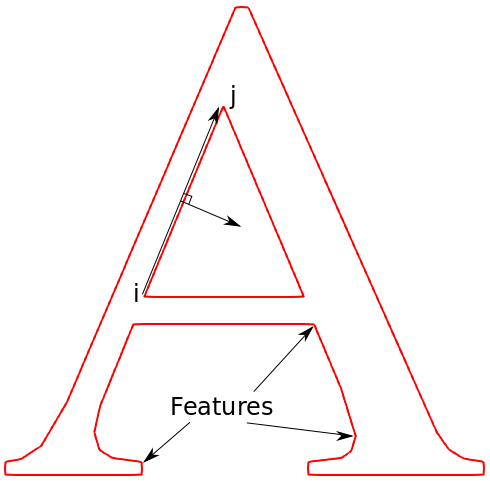
\includegraphics[width=0.24\textwidth]{a_polyline_info.png}
  \label{f:polyline}}
 \subfigure[~]{
  
\includegraphics[width=0.72\textwidth]{a_grid.png}
  \label{f:grid}}
\caption{ (a) An example of complex polyline with holes and sharp features. This corresponds to the Input to be meshed (\href{https://github.com/jaillet/MixedQuadTree/blob/master/data/a.poly}{source: a.poly}) . (b) The embedding (poorly defined...) initial quadrants structure. }
\label{fig:boundary}
\end{figure}

%---------------------------
\subsection {Polyline as Input boundary}

A \textbf{Polyline} is composed of (Fig.~\ref{f:polyline}):
\begin{itemize}
\item a vector of  \textbf{3DPoint}, with coordinates, that are all lying inside the \textbf{BoundingBox} of the Polyline,
\item and their associated angle. If the angle is not lying in the range $[MinAngle=175,MaxAngle=185]$, then it's considered as a sharp point, and called  a \textbf{Feature} in the remaining.
\item a vector of \textbf{PolyEdge}, each one defined by the indexes of the extremity' nodes, and a normal. By convention, the normal is not normed and is pointing out the Input. For an oriented edge $(i,j)$, its right side will be outside and its left side inside. Thus, the Input must be defined by closed sets of connecting edges with counter-clockwise orientation. This way, holes may be simply created.
\end{itemize}
The format for Input file might be either \verb?.poly? as described on the \href{https://www.cs.cmu.edu/~quake/triangle.poly.html}{Triangle\_1.6 website}; find an example here: \href{https://github.com/jaillet/MixedQuadTree/blob/master/data/unit\_square.poly}{unit\_square.poly}.
It could also be defined as \verb?.mdl? file, see \href{https://github.com/jaillet/MixedQuadTree/blob/master/data/unit\_square.mdl}{unit\_square.mdl}. More examples in the \href{https://github.com/jaillet/MixedQuadTree/blob/master/data/}{data} directory.

\textbf{Remarque:} \texttt{.poly} files could by displayed using the \href{https://www.cs.cmu.edu/~quake/showme.html}{ShowMe}  that comes with \textit{Triangle} software. But for practical reasons, the mesher could generate also \texttt{\_poly.vtk} files to ease visualization of the Polyline in the open-source and multi-platform \href{https://www.paraview.org/}{ParaView} suite (with option \texttt{-v}).

%---------------------------
\subsection{Quadrant as support of surface mesh}

The other important structure is the \textbf{Quadrant}:
\begin{itemize}
\item is composed of a \textit{pointindex}, vector of 4 corner indices in a vector of \textbf{MeshPoint}: Note here that MeshPoint is embedding a previously seen \textbf{3DPoint}, as well as some information describing its state. More details below.
\item When the Quadrant is subdivided into non quadrant elements (in Transitions for example), it contains a vector of \textit{sub\_elements}, each one described by a vector of indexes as presented right above.
\item It also contains a list of intersecting \textbf{PolyEdges}, and intersecting \textbf{Features}. These informations are useful to speed up the inside/outside discrimination for the Quadrant or to better handle the boundary and surface elements, for example.
\item and some additional data, for processing purpose that will be described later.
\end{itemize}

Along with the Quadrant, comes the \textbf{QuadEdge}:
\begin{itemize}
\item defined by 3 indices, the 2 extremities and potential \textit{midpoint} when this edge is split.
\end{itemize}

And finally, the \textbf{MeshPoint}:
\begin{itemize}
\item that is embedding a 3DPoint, as coordinates of the Quadrant's corners, referenced as indexes.
\item MeshPoint are conversely connected to Quadrant by an index map of \textit{elements}, referencing all the Quadrants having this point as corner.
\item it also is the support for some crucial processing information on it's \textit{state}, merged in a single byte: the point is \verb?inside?, has been \verb?projected?, is representing a \verb?feature?, has been previously \verb?checked?, etc\ldots  
\end{itemize}

These three structures will be used together along with the Polyline by the \textbf{Mesher}, that will construct them gradually:
\begin{itemize}
\item a vector of \textbf{MeshPoint},
\item a vector of \textbf{Quadrant},
\item a set of \textbf{QuadEdge}. Note that this kind of structure is costly (quasi 30\% of the whole computation time), as insertion is done in a sorted container, but it guarantees uniqueness of the element, and reasonably fast access. By the way, it might not be exactly adapted to parallelism...
\item It also contains a list of \textbf{Refinement Regions}, which usage will be presented later on.
\end{itemize}

%---------------------------
%---------------------------
\section{Main steps of the method}
\label{sec:method}
%---------------------------
%---------------------------
This mesh generator is based on the Quad-tree technique introduced in \cite{Finkel1974}. This technique recursively split a Quadrant in a finite number of equivalent sons. For instance if the Quadrant is a square, to refine it one level means that it will be replaced by 4 new Quadrants. All of them will be sons of the replaced Quadrant in the Quad-tree structure. By allowing the use of quadrants with cut corners, this modeling technique overcomes some of the drawbacks of standard Quad-tree encoding for finite element mesh generation \cite{Yerry1983}.
In our case, Quadrants will be continuously split until a maximum provided level is reached. Quadrants lying completely outside $\mathcal{S}$ will be removed.\\

\textcolor{red}{todo: mixed-elements mesh generation, describe here the main steps of the method}

\subsection{A quadtree-based method}
\textcolor{red}{show different steps of the method: }

\begin{algorithm}[H]
\SetAlgoLined
\KwResult{A mixed-elements mesh}
  \tcc{Generating quadtree:}
 \nl \ForEach{Quadrant}{
 \Repeat {desired Refinement Level}{
 \nl {Subdivide Quadrant\label{alg:subdivide}}\; 
   \ForEach{ new Sub-Quadrant}{
   \If{Intersects Input \textit{or} Is Inside}{\nl Insert Sub-Quadrant\label{alg:insertsub}}
    }
  }
  }
  \tcc{ Creating conformal mesh:}
\nl Create balanced quadtree\; \label{alg:goto}
 \nl Apply Transition Patterns\; \label{alg:trans}
 \caption{Generation process}
 \label{alg:generate}
\end{algorithm}


\begin{enumerate}
\item subdivision, quad + ROI + off-domain quad removing
\item balanced : the resulting mesh is not balanced if one of the edges of a Quadrant is subdivided twice. In this case, subdivide the Quadrant as in Algorithm~\ref{alg:generate} step~\ref{alg:subdivide}. And repeat until the mesh is balanced.
\item transition patterns (OMP)
\end{enumerate}

\textcolor{red}{todo: describe visitors}


%---------------------------
\subsection{Refinement level: all, surface and/or region}
\label{s:refinement}
Now it is possible to introduce the most important parameter of the method: the Refinement Level (\textit{rl}).
As previously said, the method is based on Quad-tree, and this user parameter will set the level of subdivision required to reconstruct the input $\mathcal{S}$.

The different option for refinement could be:
\begin{itemize}
\item refine \textbf{all} Quadrants (\texttt{-a N}). The spitting operation will be performed over each Quadrant enclosing $\mathcal{S}$. $N$ will define the refinement level \textit{rl} for this operation. For instance, \texttt{-a 2} will split all the initial Quadrants twice, replacing them by potentially 16 new Quadrants. In reality, this is achieved level by level: first subdividing and replacing the Quadrants in 4 new ones (Algorithm \ref{alg:generate} step~\ref{alg:subdivide}), keeping only those that lay inside or that intersect $\mathcal{S}$ (step~\ref{alg:insertsub}, using again a \textit{visitor}). Then, only those ones are candidates to the second level of subdivision, repeating the steps of splitting and checking of intersection on sub-Quadrants (Fig.~\ref{fig:pieref}). 
\item refine \textbf{surface} Quadrant \texttt{-s N}. The  splitting  operation  will  be  performed  over  each Quadrant  that  intersects  a  section  of $\mathcal{S}$.  For  instance, \texttt{-s  2} will  split  all  the  initial  Quadrants into  4  new  ones  and  then,  only  the  Quadrants  that  still  intersect $\mathcal{S}$ will  be  split  in 4  more, still keeping only intersecting ones (Fig.~\ref{fig:pierefs})
\item (\textcolor{red}{not tested yet in 2D!}) refine by \textbf{block} \texttt{-b} followed by the name of file where some block regions are specified. A block is defined by 2 points: $(min_x, min_y,min_z), ((max_x, max_y,max_z)$ and a refinement level \textit{rl} to be applied over the Quadrants that intersect this block. This is a text file where first we specify the number of blocks and then we detail each one of them. An example with 2 regions is now provided:\\
%
\begin{minipage}{0.2\textwidth}
\begin{tcolorbox}
\begin{verbatim}
n_regions 2
0 0 0
10 10 0
5
0 0 0
20 20 0
4
\end{verbatim}
\end{tcolorbox}
\end{minipage}
\hfill
\begin{minipage}[c]{0.65\textwidth}
In this 2D case, $min_z$ and $max_z$ are mandatory for compatibility reasons with the 3D format, but will not be used. Thus, the portion of $\mathcal{S}$ intersecting the quadrangle $(0,0) \to (10,10)$ will be refined to level 5 and the complement inside the block $(0,0) \to (20,20)$ that intersects $\mathcal{S}$ will be refined to level 4.\\[0.2cm]
\end{minipage}
\item (\textcolor{red}{not tested yet in 2D!}) refine Quadrants laying in a specific \textbf{region} \texttt{-r}. Its followed by 2 arguments: the name of file where another input surface is specified in \texttt{mdl} format and a \textit{rl}. All the Quadrants inside $\mathcal{S}$ and the specified region will be refined to \textit{rl}. %Note that this geometry can be any closed triangle mesh, for instance a tetrahedron. Also note that mesh generation time will be directly influenced by the number of triangle faces the input meshes have. In order to accelerate the process you should use as less triangles as possible that correctly define the input domains and regions. Let us say that the mesh called \texttt{myregion.mdl} intersects a portion of $\mathcal{S}$, then the instruction: \texttt{-r myregion.mdl 5} will refine to level 5 all the octants in that region. The last point regarding this option is automatic rotation. The code will compute the ``dominant normals'' of the input region and will try to align them with referential axes. This transformation will also be applied to $\mathcal{S}$. Once the mesh is generated, the inverse transformation will be applied to the output so the domain is well represented.
\end{itemize}

Finally, note that large meshes can be produced with a small value for $N$. For instance, if the starting point is only one cube and we set \texttt{N=10}, the code may produce up to $4^{10} = 1,048,576$ elements.

Of course, all these switches might be combined (as in Fig.~\ref{fig:pierefs}) to produce flexible tools and comply with the user requirements. If a Quadrant belongs to more than one refinement region (no matter the type of it), it will be refined to maximum level among those regions.\\

The \textbf{Visitor Pattern} has been implemented to circulate (\textit{visit}) the Quadrants and determine whether they should be split or not (\textit{accept}).

\textcolor{red}{todo: describe visitors}

%
\begin{figure}[htb]
\centering
 \subfigure[~]{
  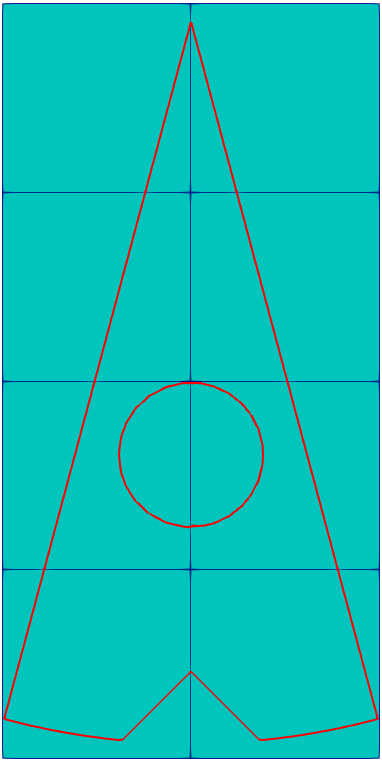
\includegraphics[width=0.14\textwidth]{pie_refined1.png}
  \label{f:pieref1}
 }
\centering
 \subfigure[~]{
  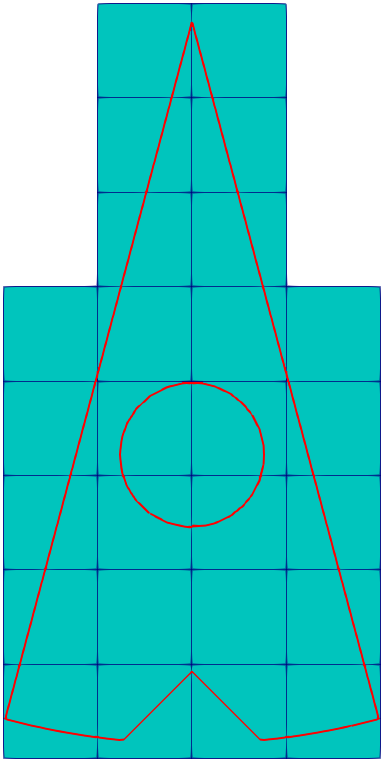
\includegraphics[width=0.14\textwidth]{pie_refined2.png}
  \label{f:pieref2}
 }
\centering
 \subfigure[~]{
  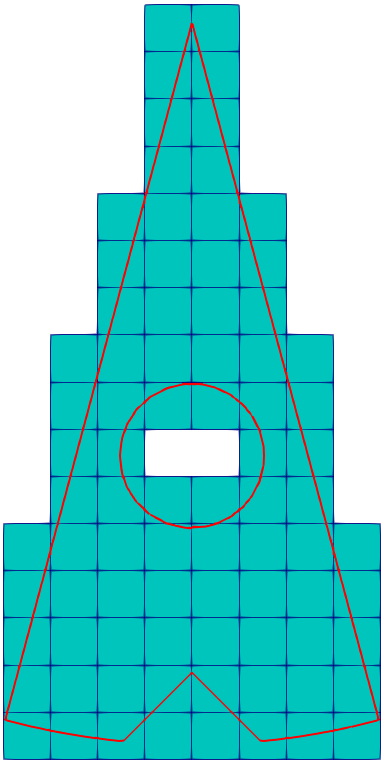
\includegraphics[width=0.14\textwidth]{pie_refined3.png}
  \label{f:pieref3}
 }
\centering
 \subfigure[~]{
  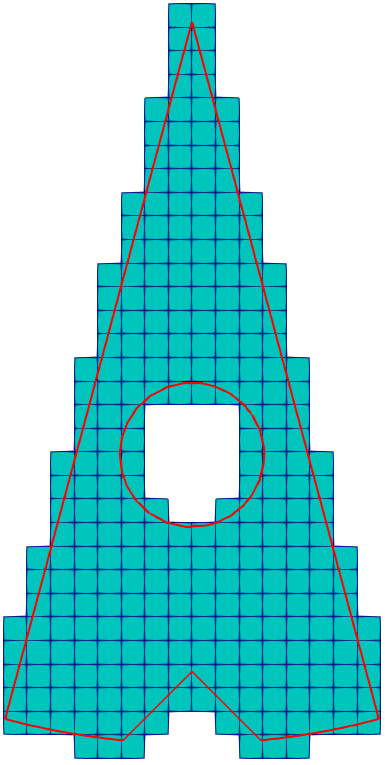
\includegraphics[width=0.14\textwidth]{pie_refined4.png}
  \label{f:pieref4}
 }
\centering
 \subfigure[~]{
  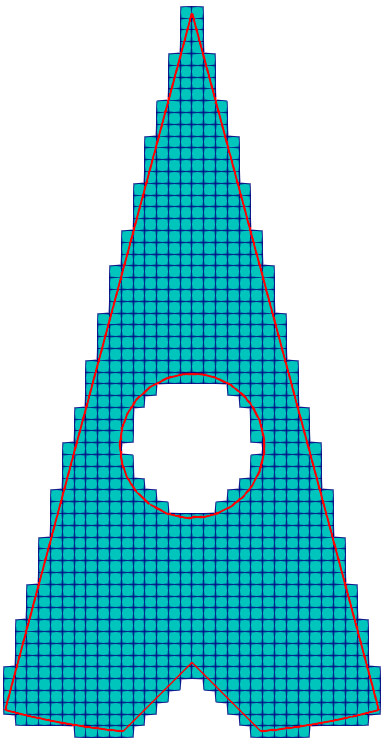
\includegraphics[width=0.14\textwidth]{pie_refined5.png}
  \label{f:pieref5}
 }
\centering
 \subfigure[~]{
  
\includegraphics[width=0.14\textwidth]{pie_refined6.png}
  \label{f:pieref6}
 }
 \caption{Effect of the refinement level applied on the complete structure (\texttt{-a N} switch, with \texttt{N=1..6})}
\label{fig:pieref}
\end{figure}
%
\begin{figure}[htb]
\centering
 \subfigure[~]{
  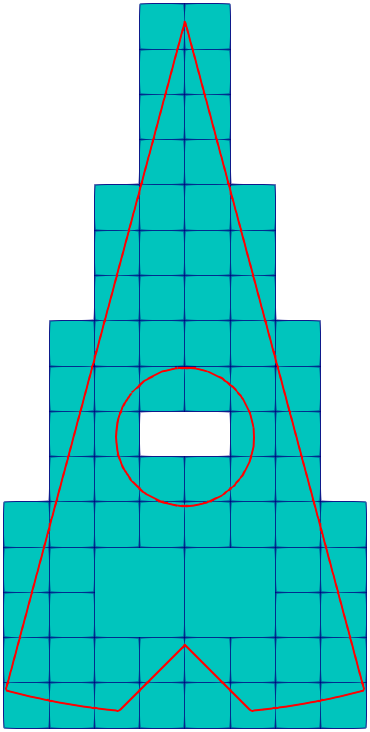
\includegraphics[width=0.22\textwidth]{pie_refined2s3.png}
  \label{f:pierefs3}
 }
\centering
 \subfigure[~]{
  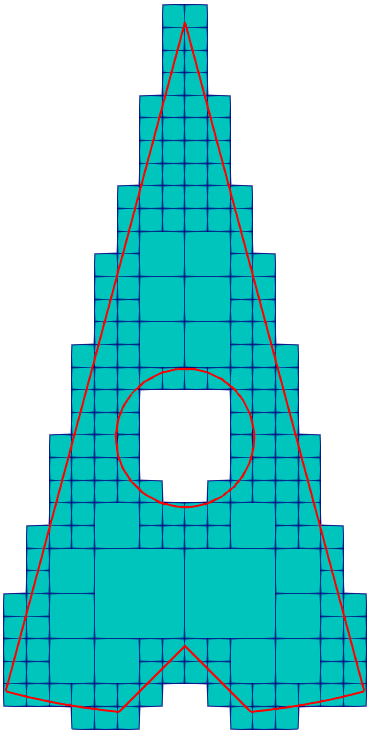
\includegraphics[width=0.22\textwidth]{pie_refined2s4.png}
  \label{f:pierefs4}
 }
\centering
 \subfigure[~]{
  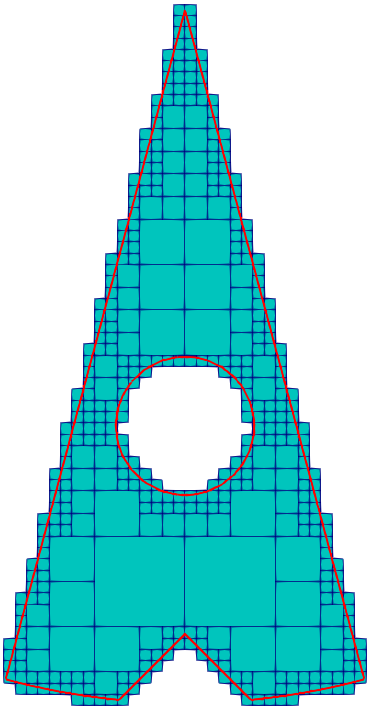
\includegraphics[width=0.22\textwidth]{pie_refined2s5.png}
  \label{f:pierefs5}
 }
\centering
 \subfigure[~]{
  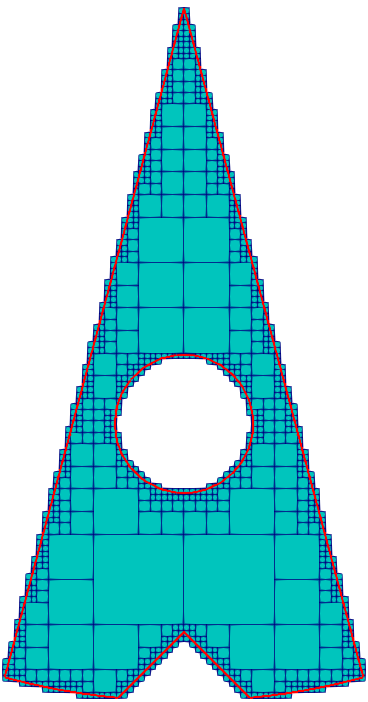
\includegraphics[width=0.22\textwidth]{pie_refined2s6.png}
  \label{f:pierefs6}
 }
 \caption{Effect of combined refinement levels, with level 2 applied on the complete structure (\texttt{-a 2} switch), and incremental refinement (\texttt{-s N} switch, with \texttt{N=3..6}) only applied on surface quadrants.}
\label{fig:pierefs}
\end{figure}

%---------------------------
\subsection{Balancing the mesh}
A Quad mesh is said \textit{balanced} when there is at most a difference of 1 level of subdivision between any two adjacent elements (step~\ref{alg:goto}). In practice, this is determined by checking whether a Quadrant contains at least one QuadEdge that is subdivided twice as in Algorithm~\ref{alg:generate} step~\ref{alg:subdivide}. Thus, for each Quadrant, every QuadEdge is checked. If one of them is subdivided, then the 2 sub-edges must be checked. Note that the \textit{search} and \textit{access} operations on QuadEdges are accelerated by the ordered set container. But whether this data structure is adapted to parallel computing is a good question\ldots

%
\begin{figure}[htb]
\centering
 \subfigure[~]{
  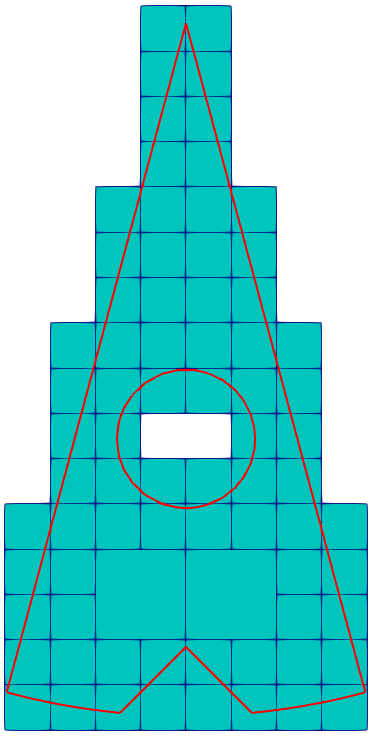
\includegraphics[width=0.22\textwidth]{pie_balanced2s3.png}
  \label{f:piebals3}
 }
\centering
 \subfigure[~]{
  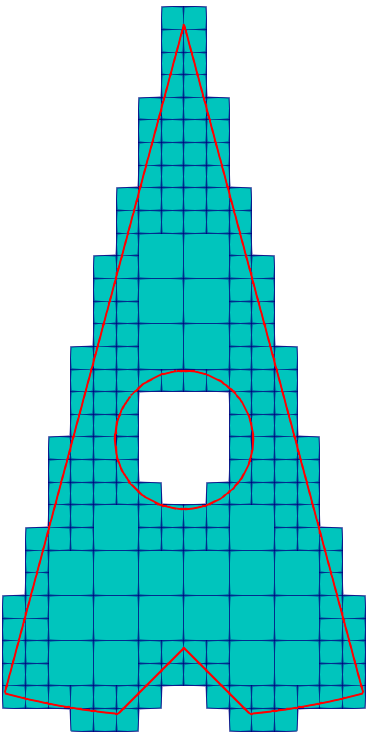
\includegraphics[width=0.22\textwidth]{pie_balanced2s4.png}
  \label{f:piebals4}
 }
\centering
 \subfigure[~]{
  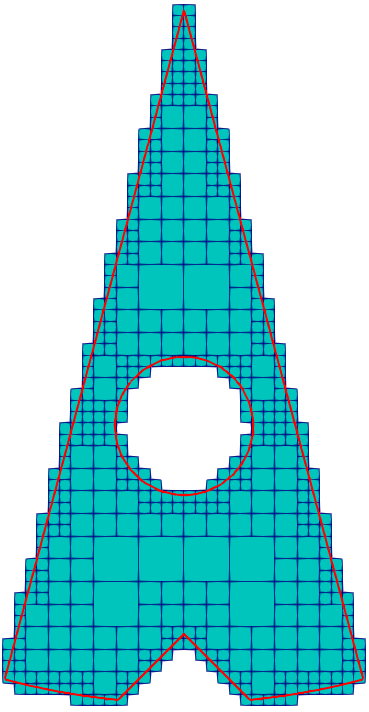
\includegraphics[width=0.22\textwidth]{pie_balanced2s5.png}
  \label{f:piebals5}
 }
\centering
 \subfigure[~]{
  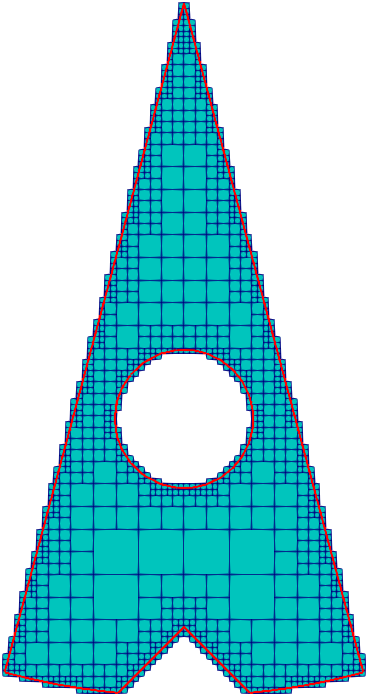
\includegraphics[width=0.22\textwidth]{pie_balanced2s6.png}
  \label{f:piebals6}
 }
 \caption{After the balancing step of previously refined mesh (sec.~\ref{s:refinement}). Note that in the first case, nothing is to be done.}
\label{fig:piebals}
\end{figure}

%---------------------------
\subsection{Transition patterns}
\label{sec:transpat}
%
Now the mesh is balanced, we need to handle transitions between Quadrants, to produce a \textit{conformal mesh}, when the elements exactly share nodes and edges. This technique is known to save time during the computation, and also to avoid node interpolation errors.
If 2 adjacent Quadrants have the same refinement level, then there is nothing to do. Otherwise, the less refined Quadrant must be treated. Again, in practice, this is determined by checking whether a Quadrant contains at least one QuadEdge that is subdivided (step~\ref{alg:trans}).

For the Transition, the chosen technique was to apply a Pattern corresponding to the  number and relative position of the refined QuadEdges. In 2D, there are only 6 cases to consider (Fig.~\ref{fig:transitionpatterns}). Note that:
\begin{itemize}
\item newly created internal edges (red lines in Fig.~\ref{fig:transitionpatterns}) are not of type QuadEdge. In that sense, they could not be subdivided again, and do not participate in the remaining of the subdivision process. They are indirectly stored as sub-elements, ie. a list of connected nodes (indexes, to be more precise),
\item all patterns are producing good shaped sub-elements,
\item and that the last one could have been simplified into 4 sub-squares, but that will require one additional middle vertex. This choice could be reconsidered if the number of elements matters more than number of points, or to improve quality, or to better handle Quadrants with Features.
\end{itemize}
%
\begin{figure}[htb]
\centering
  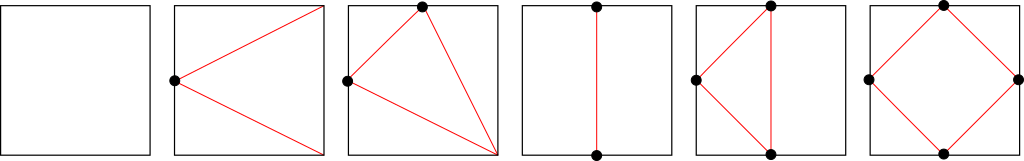
\includegraphics[width=0.84\textwidth]{transitionPatterns.png}
 \caption{All possible configurations for transition patterns in 2D. Black dots represent an edge subdivision, while red lines draw the internal edges of the Quadrant sub-elements.}
\label{fig:transitionpatterns}
\end{figure}
%
\begin{figure}[htb]
\centering
 \subfigure[~]{
  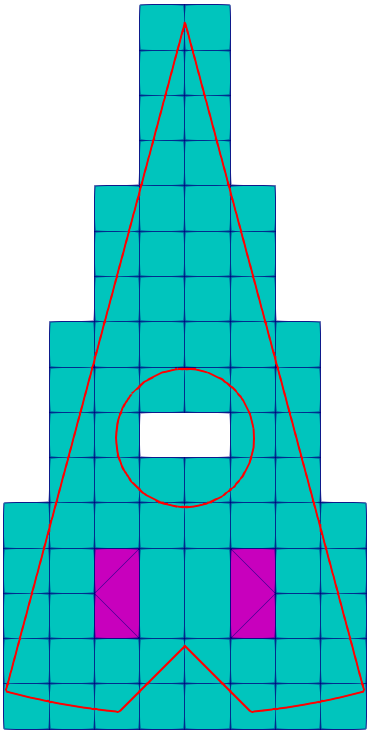
\includegraphics[width=0.22\textwidth]{pie_transition2s3.png}
  \label{f:pietranss3}
 }
\centering
 \subfigure[~]{
  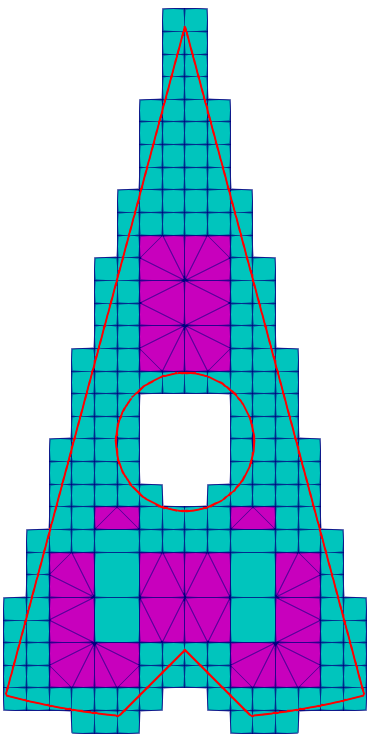
\includegraphics[width=0.22\textwidth]{pie_transition2s4.png}
  \label{f:pietranss4}
 }
\centering
 \subfigure[~]{
  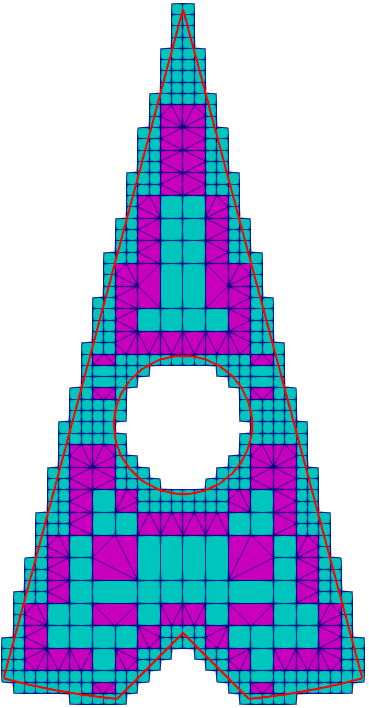
\includegraphics[width=0.22\textwidth]{pie_transition2s5.png}
  \label{f:pietranss5}
 }
\centering
 \subfigure[~]{
  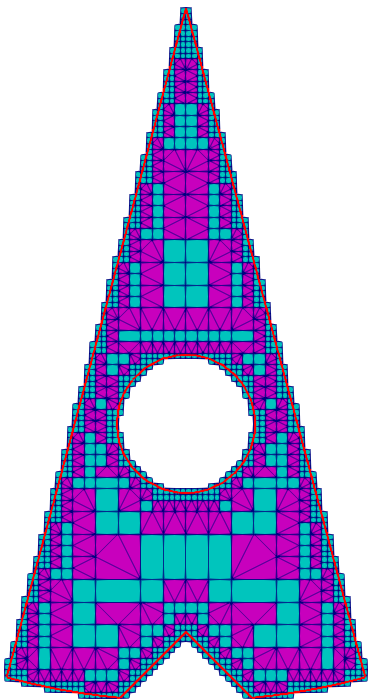
\includegraphics[width=0.22\textwidth]{pie_transition2s6.png}
  \label{f:pietranss6}
 }
 \caption{After the transition step. Note that the more difference between levels, the more transition patterns are used\ldots}
\label{fig:pietranss}
\end{figure}

%---------------------------
%---------------------------
\section{Fitting quadrants to Input Polyline}
\label{sec:method}
%---------------------------
%---------------------------

As seen previously in section~\ref{sec:method}, Quadrants are well suited to decompose the input  domain $\mathcal{S}$ into a set of Elements. However, you may notice that the Boundaries are not exactly fitted when PolyEdges are not aligned with the Quadrants border, unless you use a very fine subdivision\ldots that is generally unwanted to avoid generating a huge amount of Elements.

Thus, following the same approach as for Transition Patterns (see~\ref{sec:transpat}), the Boundary Elements will be treated with \textit{Surface Patterns}, as described in Algorithm~\ref{alg:surfacefitting}.\\

\begin{algorithm}[H]
%
\setcounter{AlgoLine}{-1}
\SetAlgoLined
\KwResult{A mixed-elements mesh}
  \tcc{Preprocess:}
\nl   Handle Boundary\; \label{alg:bound2}
 \tcc{Generating quadtree:}
\nl \ForEach{Quadrant}{
 \Repeat {desired Refinement Level}{
 \nl Subdivide Quadrant\; \label{alg:subdivide2}
   \ForEach{ new Sub-Quadrant}{
   \If{Intersects Input \textit{or} Is Inside}{\nl Insert Sub-Quadrant \label{alg:insertsub2}}
    }
  }
  }
   \tcc{ Creating conformal mesh:}
\nl Create balanced quadtree\; \label{alg:goto2}
 \nl Apply Transition Patterns\;
 \tcc{Input surface fitting:}
 \nl Detect Features in Input\;
 \nl  Project Close to Boundary Intern Nodes\; \label{alg:closeto2}
  \nl Remove Outside Quadrant\; \label{alg:remsur2}
  \nl Shrink Extern Nodes to Boundary\; \label{alg:shrink2}
 \nl Apply Surface Patterns\; \label{alg:surfpat2}
 \caption{Generation process and Input surface fitting}
 \label{alg:surfacefitting}
\end{algorithm}

%---------------------------
\subsection{Boundary and sharp features handling}
\label{sec:boundary}

\textcolor{red}{preprocessing}
This stage is a preprocessing 

\begin{enumerate}
\item        // test1: if nb Features $>= 2$
        // first condition is optimization if NbFeatures has been already computed
\item        // test2: if $distFProjectionFeature > distMax$ for each node
        // done: compute distMax before...
\item        // test3: if the number of intersection of the Polyline and Quadrant edge $>= 3$
\end{enumerate}
The result for the \textit{A} and \text{Pie} Polyline is shown on Fig.~\ref{fig:boundary}, where it can be appreciated that subdivision only occurred where required and is driven by the Input Polyline characteristics.

 \begin{figure}[htb]
\centering
 \subfigure[~]{
  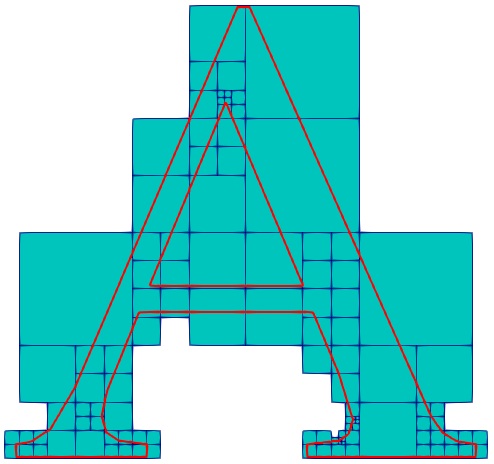
\includegraphics[width=0.6\textwidth]{a_boundary.png}
  \label{f:aboundary}
 }
 \subfigure[~]{
  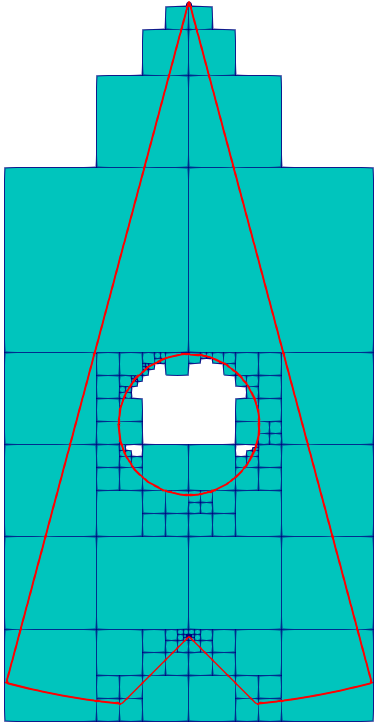
\includegraphics[width=0.3\textwidth]{pie_boundary.png}
  \label{f:pieboundary}
 }
\caption{After preprocessing for Boundary handling, leading to a better representation of the Input Polyline.}
\label{fig:boundary}
\end{figure}

\textcolor{red}{setting, or not, a refinement level for Boundary handling}
This preprocessing will now serve as input for Algorithm~\ref{alg:generate} or \ref{alg:surfacefitting}. 


%---------------------------
\subsection{Generating first quadrants over boundary prepared mesh}
This is exactly the same as in Algorithm~\ref{alg:generate}. The only difference is the initial Quadrant list, that as been prepared as described in section~\ref{sec:boundary}

\begin{figure}[htb]
\centering
 \subfigure[~]{
  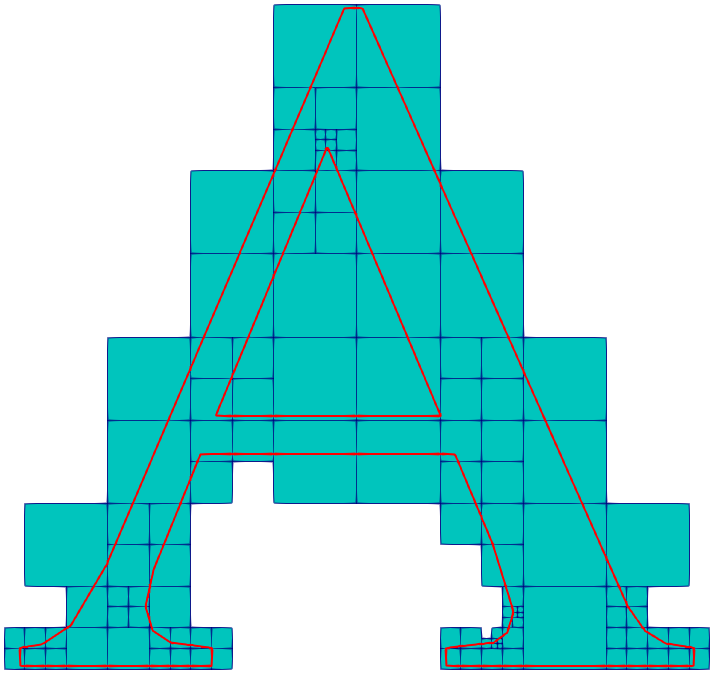
\includegraphics[width=0.31\textwidth]{a3_boundary_refined.png}
  \label{f:boundaryref3}
 }
  \subfigure[~]{
  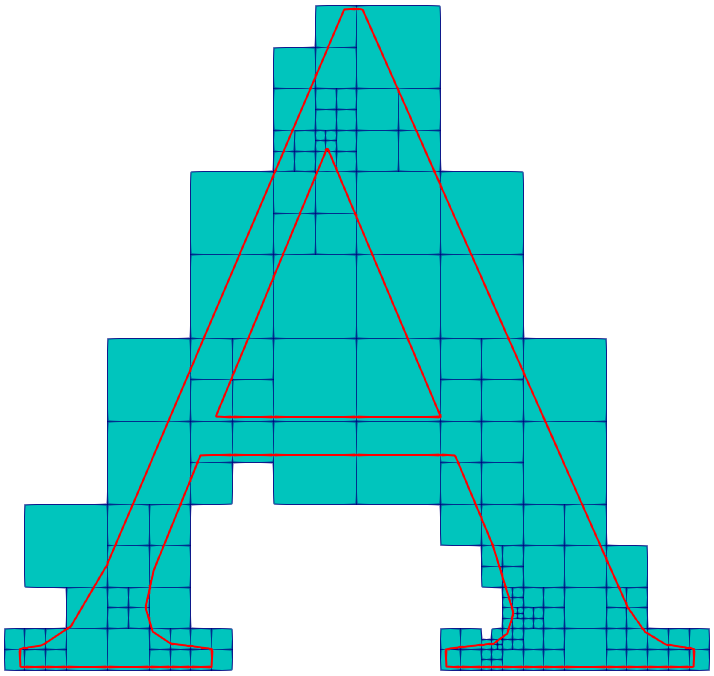
\includegraphics[width=0.31\textwidth]{a3_boundary_balanced.png}
  \label{f:boundarybal3}
 }
 \subfigure[~]{
  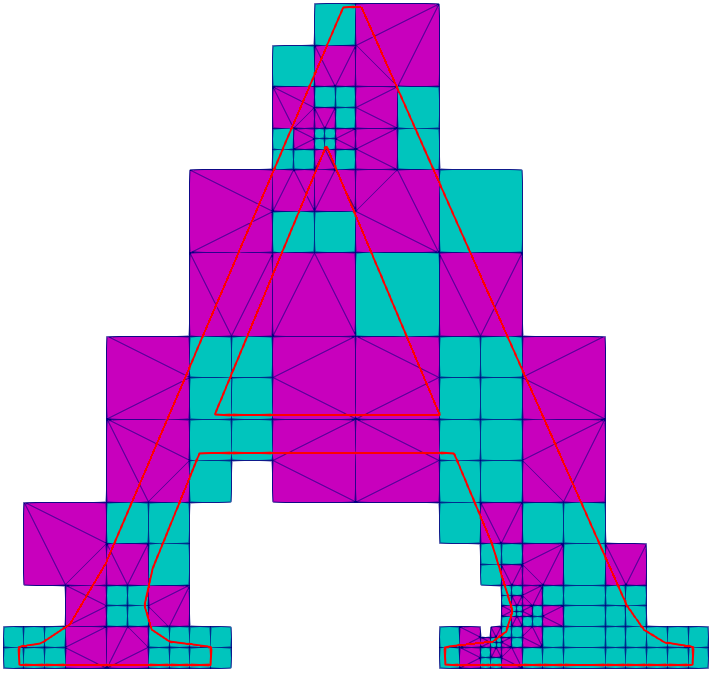
\includegraphics[width=0.31\textwidth]{a3_boundary_transition.png}
  \label{f:boundarytrans3}
 }
 \caption{After refinement level 3, balancing and transition steps (see Algorithm~\ref{alg:generate}).}
\label{fig:generate3}
\end{figure}

\begin{figure}[htb]
\centering
 \subfigure[~]{
  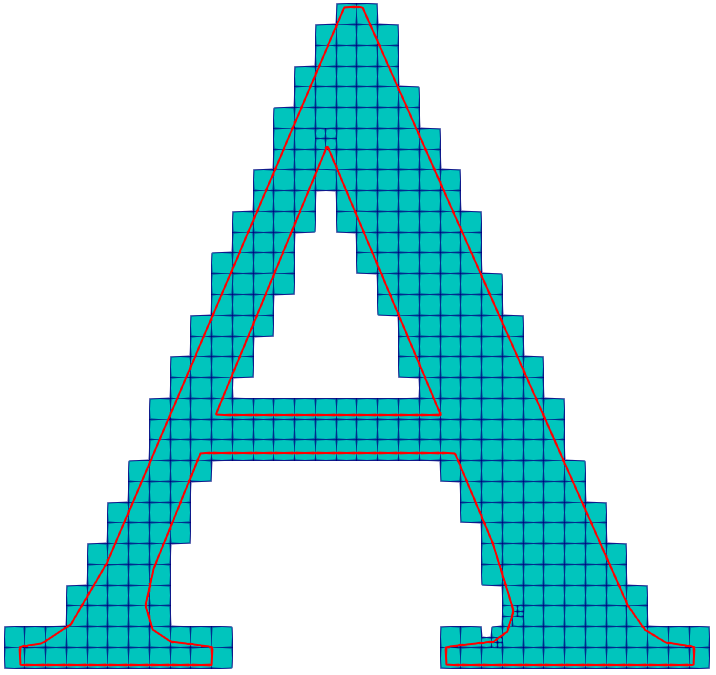
\includegraphics[width=0.31\textwidth]{a5_boundary_refined.png}
  \label{f:boundaryref5}
 }
  \subfigure[~]{
  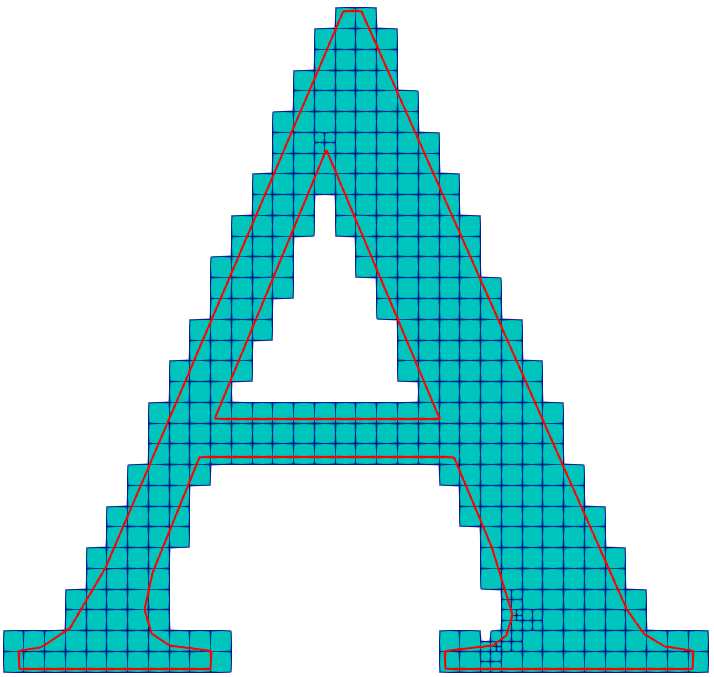
\includegraphics[width=0.31\textwidth]{a5_boundary_balanced.png}
  \label{f:boundarybal5}
 }
 \subfigure[~]{
  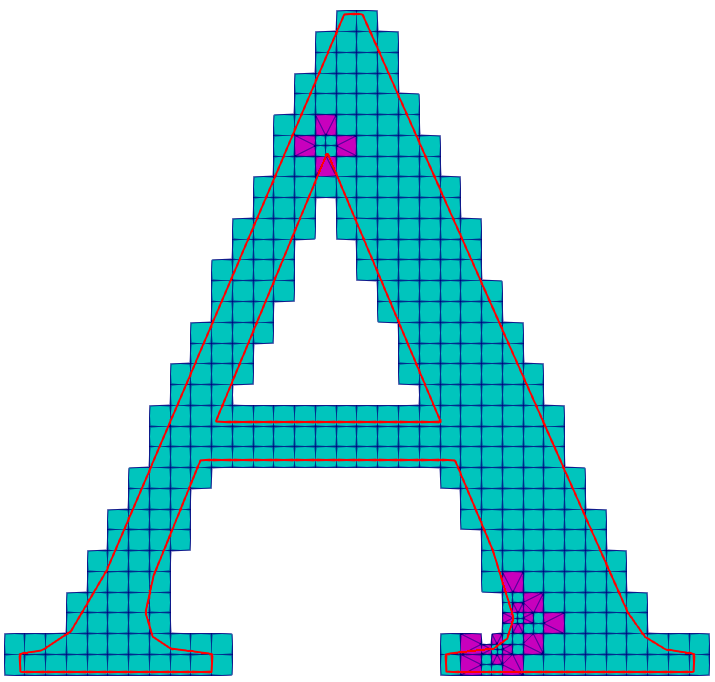
\includegraphics[width=0.31\textwidth]{a5_boundary_transition.png}
  \label{f:boundarytrans5}
 }
 \caption{After refinement level 5, balancing and transition steps (see Algorithm~\ref{alg:generate}).}
\label{fig:generate5}
\end{figure}

\begin{figure}[htb]
\centering
 \subfigure[~]{
  
\includegraphics[width=0.31\textwidth]{a7_boundary_refined.png}
  \label{f:boundaryref7}
 }
  \subfigure[~]{
  
\includegraphics[width=0.31\textwidth]{a7_boundary_balanced.png}
  \label{f:boundarybal7}
 }
 \subfigure[~]{
  
\includegraphics[width=0.31\textwidth]{a7_boundary_transition.png}
  \label{f:boundarytrans7}
 }
 \caption{After refinement level 7, balancing and transition steps (see Algorithm~\ref{alg:generate}).}
\label{fig:generate7}
\end{figure}


%---------------------------
\subsection{Handling Input surface}

\textcolor{red}{describe sub-algorithms for each step, in particular the Surface Patterns that are the main contribution of the method and most delicate step\ldots}

\begin{figure}[htb]
\centering
 \subfigure[~]{
  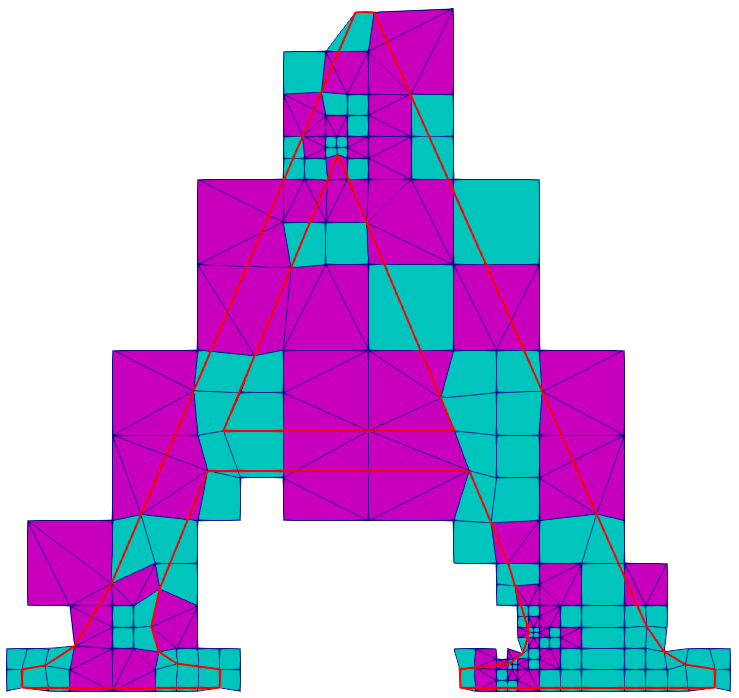
\includegraphics[width=0.33\textwidth]{a_boundary_projectinteriorcloseto3.png}
  \label{f:boundaryclose3}
 }
 \subfigure[~]{
  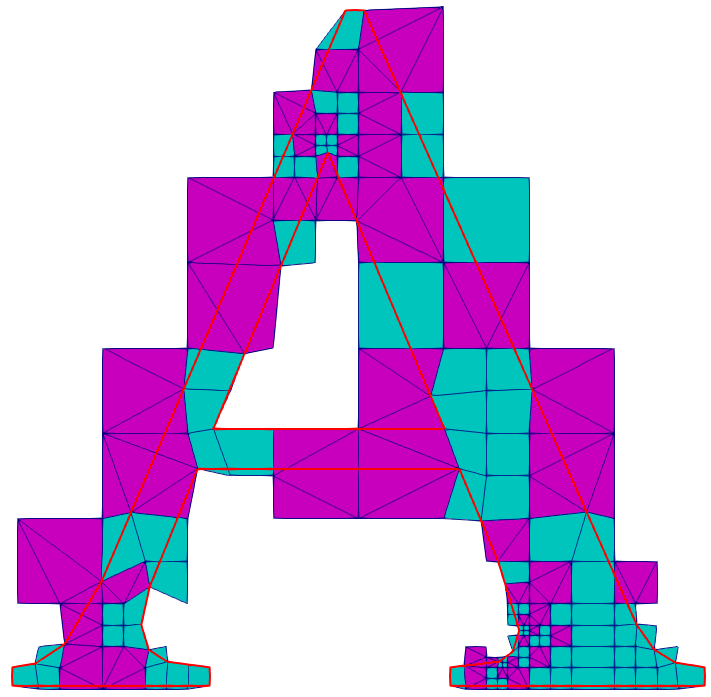
\includegraphics[width=0.33\textwidth]{a_boundary_removesurface3.png}
  \label{f:boundaryrem3}
 }\\
  \subfigure[~]{
  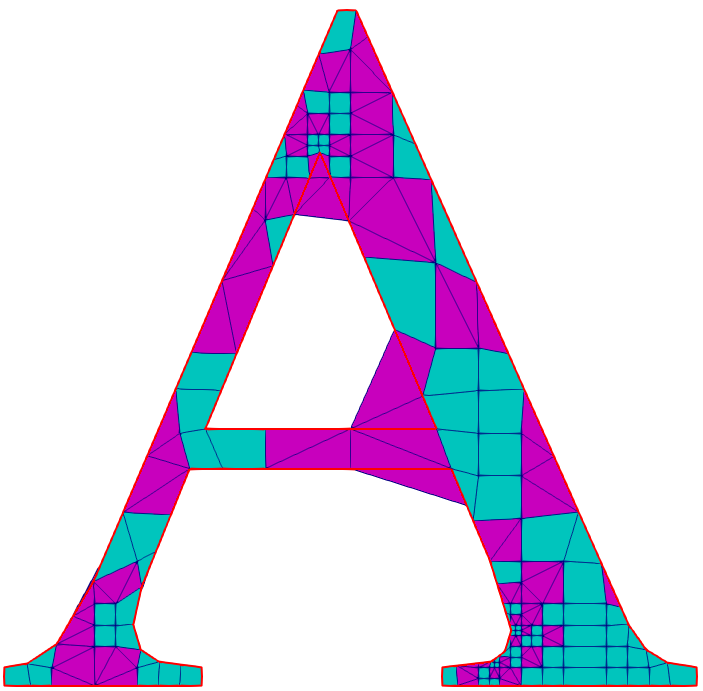
\includegraphics[width=0.33\textwidth]{a_boundary_shrinkexterior3.png}
  \label{f:boundaryshrink3}
 }
  \subfigure[~]{
  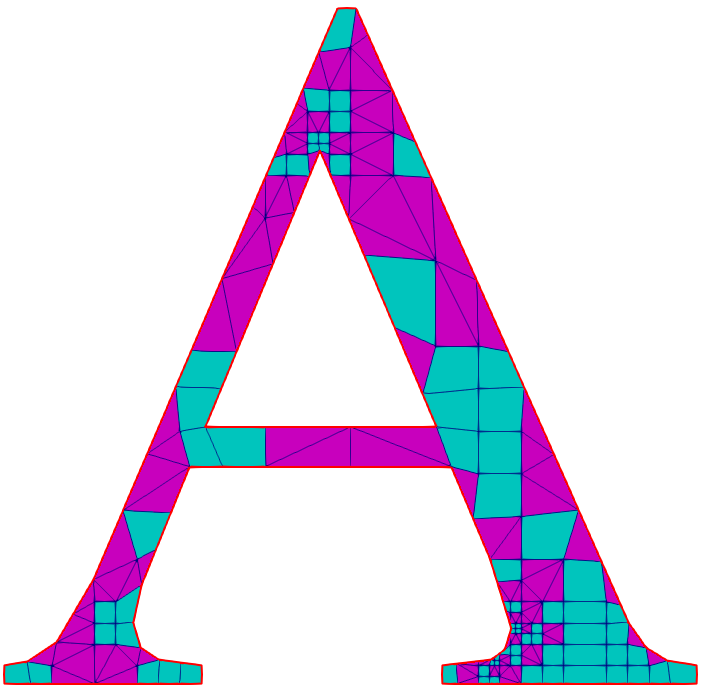
\includegraphics[width=0.33\textwidth]{a_boundary_surfacepatterns3.png}
  \label{f:boundarysurf3}
 }
 \caption{Algorithm~\ref{alg:surfacefitting}, level 3. After projecting interior points close to boundary (step~\ref{alg:closeto2}), removing exterior quadrants (step~\ref{alg:remsur2}), projection external nodes to boundary (step~\ref{alg:shrink2}) and finally applying Surface Patterns (step~\ref{alg:surfpat2}).}
\label{fig:surfacehandling3}
\end{figure}
%
\begin{figure}[htb]
\centering
 \subfigure[~]{
  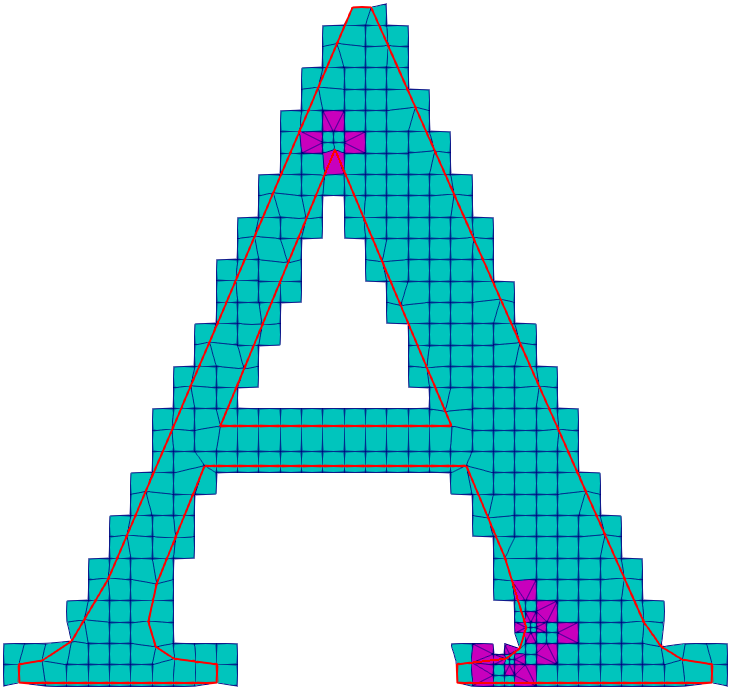
\includegraphics[width=0.33\textwidth]{a_boundary_projectinteriorcloseto5.png}
  \label{f:boundaryclose5}
 }
 \subfigure[~]{
  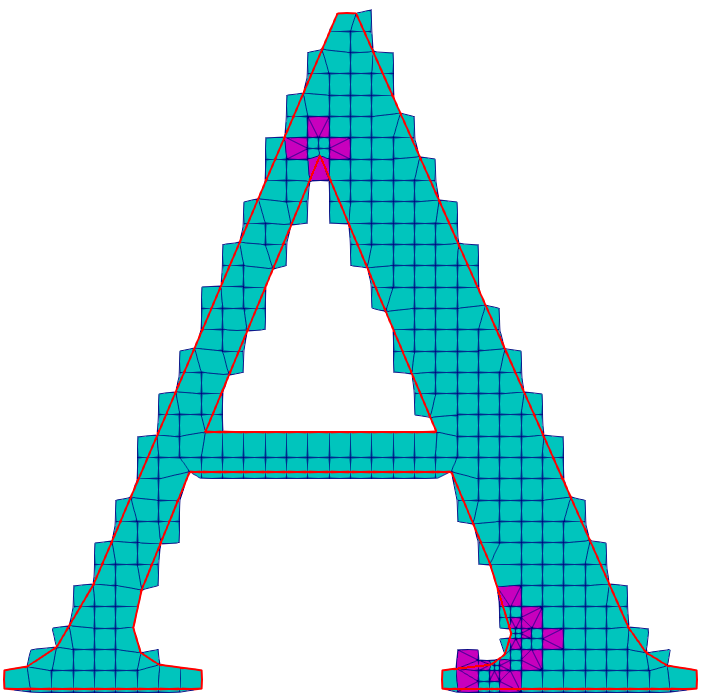
\includegraphics[width=0.33\textwidth]{a_boundary_removesurface5.png}
  \label{f:boundaryrem5}
 }
 \\
  \subfigure[~]{
  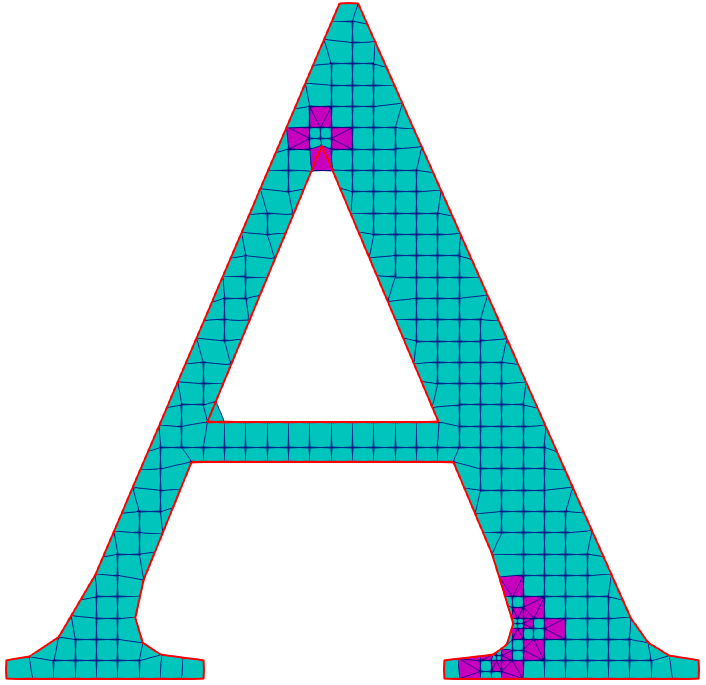
\includegraphics[width=0.33\textwidth]{a_boundary_shrinkexterior5.png}
  \label{f:boundaryshrink5}
 }
  \subfigure[~]{
  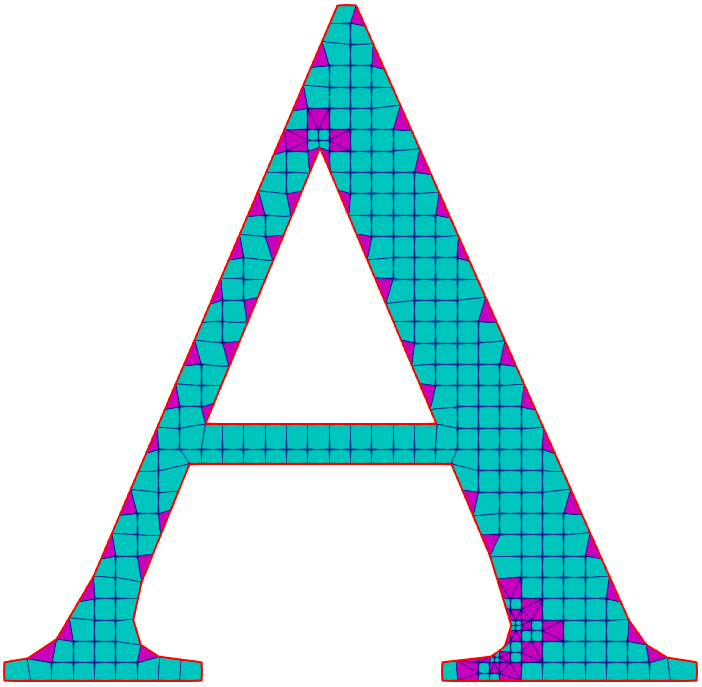
\includegraphics[width=0.33\textwidth]{a_boundary_surfacepatterns5.png}
  \label{f:boundarysurf5}
 }
 \caption{Algorithm~\ref{alg:surfacefitting}, level 5. After projecting interior points close to boundary (step~\ref{alg:closeto2}), removing exterior quadrants (step~\ref{alg:remsur2}), projection external nodes to boundary (step~\ref{alg:shrink2}) and finally applying Surface Patterns (step~\ref{alg:surfpat2}).}
\label{fig:surfacehandling5}
\end{figure}
%
\begin{figure}[htb]
\centering
 \subfigure[~]{
  
\includegraphics[width=0.33\textwidth]{a_boundary_projectinteriorcloseto7.png}
  \label{f:boundaryclose7}
 }
 \subfigure[~]{
  
\includegraphics[width=0.33\textwidth]{a_boundary_removesurface7.png}
  \label{f:boundaryrem7}
 }\\
  \subfigure[~]{
  
\includegraphics[width=0.33\textwidth]{a_boundary_shrinkexterior7.png}
  \label{f:boundaryshrink7}
 }
  \subfigure[~]{
  
\includegraphics[width=0.33\textwidth]{a_boundary_surfacepatterns7.png}
  \label{f:boundarysurf7}
 }
 \caption{Algorithm~\ref{alg:surfacefitting}, level 7. After projecting interior points close to boundary (step~\ref{alg:closeto2}), removing exterior quadrants (step~\ref{alg:remsur2}), projection external nodes to boundary (step~\ref{alg:shrink2}) and finally applying Surface Patterns (step~\ref{alg:surfpat2}).}
\label{fig:surfacehandling7}
\end{figure}



%---------------------------
%---------------------------
\section{Remeshing}
\label{sec:remeshing}
%---------------------------
%---------------------------
\textcolor{red}{todo description, main point is the recycling of previously generated Quad Mesh, and Quad identification for the element list to be refined.}

\begin{algorithm}[H]
\SetAlgoLined
\SetKw{kwGoto}{Goto}
\KwResult{A refined mixed-elements mesh}
  \tcc{Reconstructing quadtree}
\nl Read .oct file\;
\nl Regenerate quadtree\;
  \tcc{Refining Elements}
 \ForEach{Element to refine}{
\nl   Identify containing Quadrant\;
\nl   Subdivide Quadrant\;
   \ForEach{Sub-quadrant}{
\nl    \If{Intersect Input \textit{or} Is Inside}{Insert Sub-Quadrant}
    }
  }
   \tcc{Conformal mesh and Input surface fitting}
  \kwGoto{Algorithm \ref{alg:surfacefitting}, step \ref{alg:goto2}}
 \caption{Refinement process}
 \label{alg:refinement}
\end{algorithm}

\subsection{.oct File Format}
The mesh generation process as described in Algorithms~\ref{alg:generate} and \ref{alg:surfacefitting} will always produce a \texttt{.oct} file, describing the Quadrants structure and required additional information.\\
Note that the \texttt{.oct} extension is an oddity, kept for compatibility reasons with the 3D version. \texttt{.quad} would probably be more relevant.

Fields of the file are most of the time self-explanatory, except for Quadrants' link. This latter informs on the number of sub-elements contained in each Quadrant. It is equal to $1$ for generic Quadrants, and between $2$ and $5$ in case of Transition of Surface Quadrants, independently of the type of the element, triangle o quadrangle (as shown in Fig.~\ref{fig:transitionpatterns}). \\
Generally, after a general-purpose simulation, we get a list of Elements to be refined, and not a list of Quadrants (as the Quadrants structure is not known by the simulation). So this data allows to construct a mapping between the index of an Element, and the Quadrant that contains it. This way, we are able to determine the list of Quadrants to be subdivided by the \textit{Remeshing} step.

Besides, the Quadrant part of the file contains a list of intersected faces (\textit{ie.} edges of the Polyline). The computation of this intersection is particularly time consuming, and it is worth to be stored directly in the \texttt{.oct} file.

\begin{tcolorbox}[skin=enhanced,breakable]
\begin{verbatim}
#NbVertex #NbEdges #NbLinks #NbQuadrants

# Coordinates of the Quadrants' vertices
x y z

# Edges: vertex Indices
# with i0 i1: indices of edge' extremities
# and i2 index of the middle point of the edge
i0 i1 i2

# Quadrants links
# one line: number of Elements for each Quad
e0 ... en-1

# Quadrants data
# 2 lines for each Quad
# first line: number of corners (should be 4!)
# followed by indices of Corner's vertices and refinement level 
4 v0 v1 v2 v3 rl
# second line:  number of intersected faces (Input)
# followed by list of intersected faces
n f0 ... fn-1

# Geometric Transform
Geometric Transform
x y z # centroid coordinates
x y z # axis coordinates
\end{verbatim}
\end{tcolorbox}

\subsection{Results}

Some results are shown on Fig.~\ref{fig:refiningbox}. On each image, the bottom left element is refined. Notice how mesh is balanced and transition are created to produce a conformal mesh. Note how successive mesh refinement keeps the good quality if the elements. 
\begin{figure}[htb]
\centering
 \subfigure[~]{
  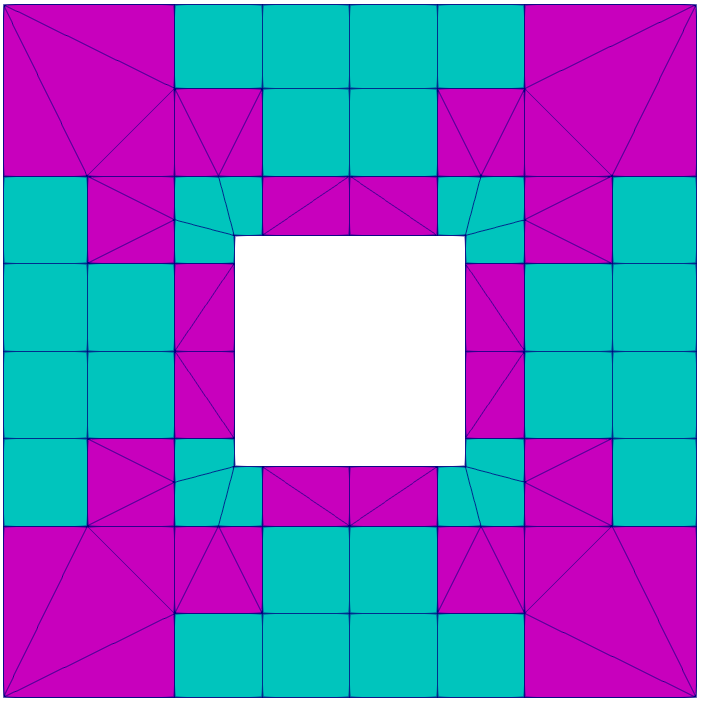
\includegraphics[width=0.31\textwidth]{box1.png}
  \label{f:box1}
 }
 \subfigure[~]{
  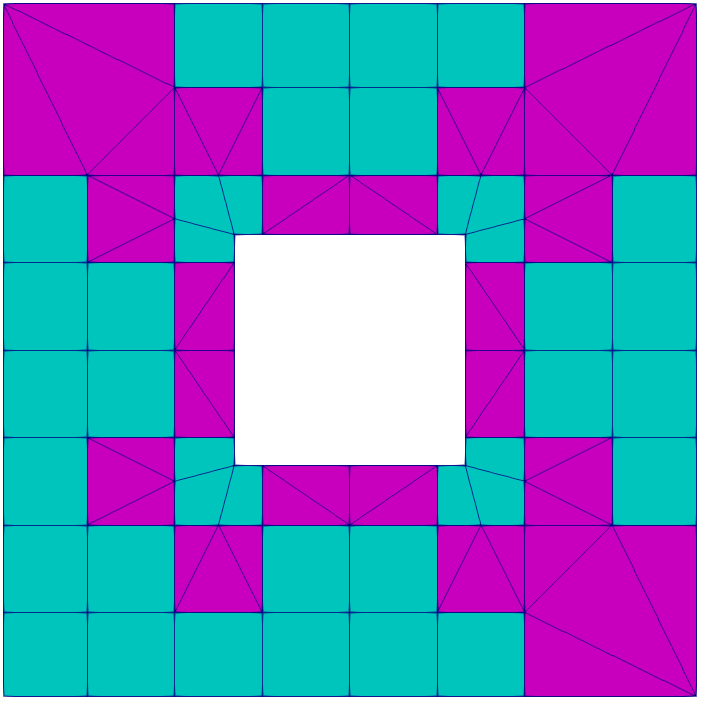
\includegraphics[width=0.31\textwidth]{box2.png}
  \label{f:box2}
 }
  \subfigure[~]{
  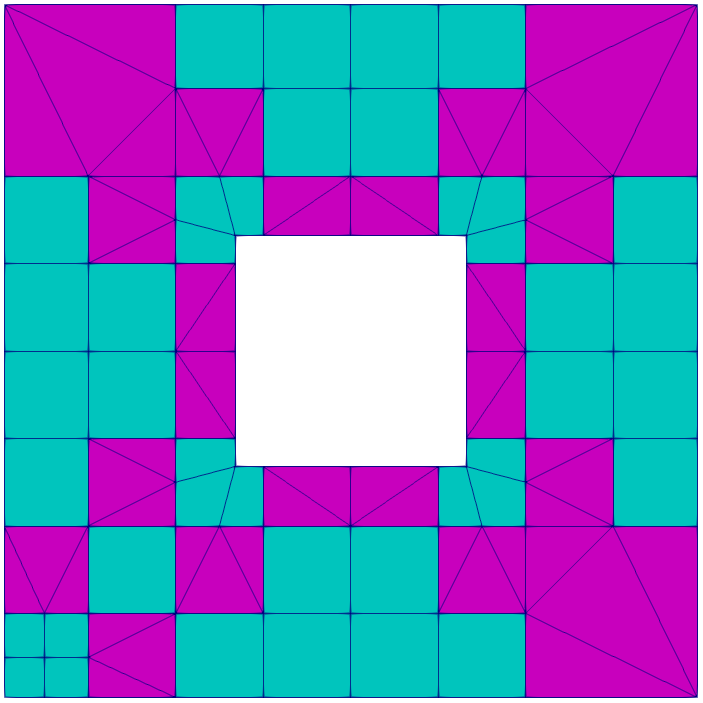
\includegraphics[width=0.31\textwidth]{box3.png}
  \label{f:box3}
 }
  \subfigure[~]{
  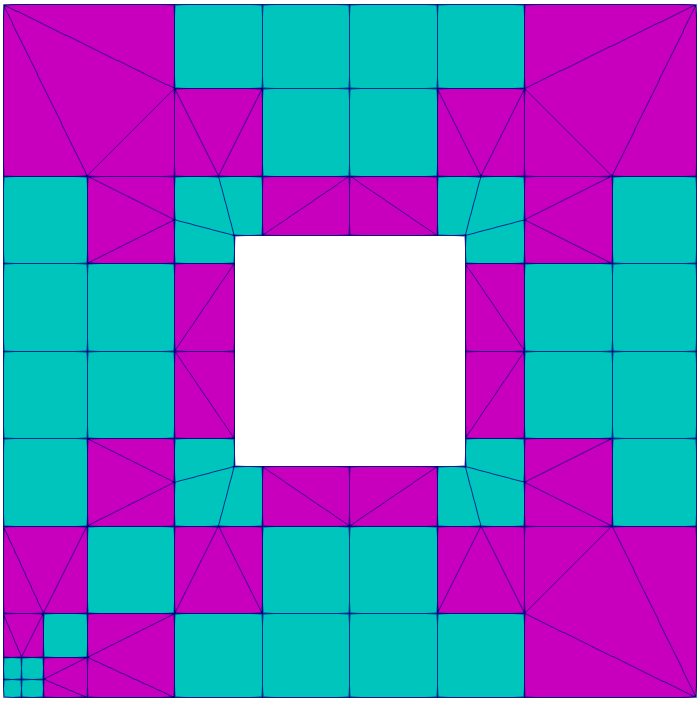
\includegraphics[width=0.31\textwidth]{box4.png}
  \label{f:box4}
 }
  \subfigure[~]{
  \includegraphics[width=0.31\textwidth]{box5.png}
  \label{f:box5}
 }
  \subfigure[~]{
  \includegraphics[width=0.31\textwidth]{box8.png}
  \label{f:box8}
 }
 \caption{Iterating on Algorithm~\ref{alg:refinement}\ . With \textit{Box} example, the bottom left element is refined once at each iteration of the algorithm. (a-c) iteration 1 to 5, (d) iteration 8.}
\label{fig:refiningbox}
\end{figure}

\begin{figure}[htb]
\centering
 \subfigure[~]{
  \includegraphics[width=0.31\textwidth]{box20.png}
  \label{f:box20}
 }
 \subfigure[~]{
  \includegraphics[width=0.31\textwidth]{box20_zoom1.png}
  \label{f:boox20z1}
 }
  \subfigure[~]{
  \includegraphics[width=0.31\textwidth]{box20_zoom2.png}
  \label{f:box20z2}
 }
 \caption{Iterating on Algorithm~\ref{alg:refinement}.  Same \textit{Box} example as Fig.~\ref{fig:refiningbox}, iteration 20. (b) Zooming once and (b) twice at the bottom left corner.}
\label{fig:refiningbox20}
\end{figure}



identify which Quad contains the element, information from file

subdivide Quad + goto subsection balanced

\textcolor{red}{
(local remeshing? neighbourhood??)
}

\textcolor{red}{
Discussion: the limitation of the currently proposed method is clearly the lack of a local remeshing process. As described right above, 
}


%---------------------------
%---------------------------
\section{Installing}
\label{install}
%---------------------------
%---------------------------

In order to install this application you will need a Unix--based system, a \texttt{c++} compiler and \texttt{cmake}. You should do the following:

%---------------------------
\subsection{Create an account on github.com}

\begin{itemize}
\item go to github.com, then 'Signup and Pricing' $\Rightarrow$ 'Free for open source' $\Rightarrow$ 'Create a free account'
\item choose Username/Email/Password and it's done
\item you can also update your account settings (website, avatar...)
\end {itemize}

%---------------------------
\subsection{Git Fork MixedQuadTree}

Let's fork the initial MixedQuadTree repository. So, once you're logged in on github:
\begin{itemize}
\item go to https://github.com/jaillet/MixedQuadTree/
\item click on the 'Fork' button
\item once the fork is finished, you'll have your own copy of MixedQuadTree with the following path: https://github.com/\textbf{yourUsername}/MixedQuadTree
\item at this URL, you're able to browse the sources, see the commit log, report issues...
\end {itemize}

%---------------------------
\subsection{Getting the program, and Compiling}

\begin{tcolorbox}{\small
\begin{verbatim}
$ git clone /https://github.com/jaillet/MixedQuadTree.git
$ cd MixedQuadTree/
$ git checkout -b develop upstream/develop (this will create a new branch and follow upstream one)
$ or (git checkout develop) once the branch has been created
$ mkdir build ; cd build
$ cmake ../src -D_CMAKE_BUILD_TYPE=Debug (or Release) // Uppercase is important
$ cmake .
$ make -j#nproc
\end{verbatim}
}\end{tcolorbox}

\subsection{Git usage}
At this point, you can edit and commit files on you branch using  the git workflow.

In order to easily access to the initial MixedQuadTree repository and stay updated with the other developers advances, you can set it as a remote repository, called 'upstream' (\href{https://help.github.com/articles/syncing-a-fork/}{github help}):


\begin{tcolorbox}
\begin{verbatim}
$ git remote add upstream git@github.com:MixedQuadTree/MixedQuadTree.git
\end{verbatim}
\end{tcolorbox}

Git remotes are great because they allows to have multiple pull/push repositories. You can see the list of your remote repositories under a shell:

\begin{tcolorbox}
\begin{verbatim}
$ git remote
$ git remote -v
\end{verbatim}
\end{tcolorbox}

At this point, you should have two remote repositories:
%
\begin{itemize}
\item origin, your own fork of the initial MixedQuadTree repository
\item upstream, the remote repository you have just added containing the initial MixedQuadTree repository
\end{itemize}

You can see the state of a remote repository called 'remotename' under a shell with the command 'git remote show remotename':
%
\begin{tcolorbox}\begin{verbatim}
$ git remote show origin
$ git remote show upstream (you can use the tab-key for auto-completion)
\end{verbatim}
\end{tcolorbox}

In the normal workflow, you can pull from the main MixedQuadTree repository (upstream)...
%
\begin{tcolorbox}\begin{verbatim}
$ git pull upstream master
\end{verbatim}
 \end{tcolorbox}

\textbf{IMPORTANT NOTE $\Rightarrow$ but only push to your own fork of MixedQuadTree (origin) !!!}

\begin{tcolorbox}\begin{verbatim}
$ git push origin master
\end{verbatim}
\end{tcolorbox}

The merge between the original repository is done by ANOTHER DEVELOPER after a \textbf{'pull request'}.
To make a 'pull request', go to \url{https://github.com/yourUsername/MixedQuadTree}, click on 'Pull Request'. Then, choose the two branches you would like to merge (master in \textit{jaillet} and your branch in \textit{origin}), write your comments and click on \textit{'Send Pull Request'}.


%---------------------------
%---------------------------
\section{Standalone program use}
\label{standalone}
%---------------------------
%---------------------------

%---------------------------
\subsection{Produce a conformal high-quality mixed--elements mesh}
\label{s:generatemesh}

To produce a mesh you must execute in a terminal the following:
%
\begin{tcolorbox}
{\small
\begin{verbatim}
$ ../mesher_roi [-option | parameters]
\end{verbatim}
}\end{tcolorbox}

If you do not indicate any option nor parameters, the program will list all the available options for you. Options for input/output:
\begin{tcolorbox}
{\small
\begin{verbatim}
    usage: ./mesher [-p] input.poly [-u] output
                    [-s] ref_level [-a] ref_level [-b] file.reg
                    [-r] input_surface rl [-option 1] .. [-option n]
    where:
      one of the parameters must be an input surface mesh in
      mdl or off format. If output name is not provided it
      will be saved in input_name.m3d. Options:
        -d input surface as .mdl file (alternative to -p).
        -s Refine Quadrants intersecting the input surface.
           Parameter ref_level is the refinement level
        -a Refine all elements in the input domain.
           Parameter ref_level is the refinement level
        -b Refine block regions provided in file file.reg
        -r Refine surface region. Will refine all the elements
           in the provided input_surface at level rl
        -q if supported (only VTK by now), write quality attributes to output file.
        -g save output mesh in GetFem format (gmf)
        -v save output mesh + input in VTK ASCII format (vtk)
        -m save output mesh in M3D ASCII format (m3d)
        -x save output mesh in GMSH ASCII format (gmsh)
        -i save output mesh in MVM ASCII format (mvm)
        -o save output mesh in OFF ASCII format (off)
\end{verbatim}
}\end{tcolorbox}


\begin{itemize}
\item \texttt{-p}: with the name of an input file (\texttt{.poly} extension) where the surface Polyline is specified. In this version of the code, only one input can be specified.
\item  \texttt{-d} input surface as .mdl file (alternative to -p).
\item \texttt{-u}: next to it comes the name of the output file. The extension (file format) will be automatically added and  it can be changed with one (or several) of  the next options \texttt{-g, -v, -m, -x, -i, -o}. \textcolor{red}{(check if default for  name and format!)}
\item \texttt{-q}: add decoration to the VTK file (must be used along with \texttt{-v}). Useful for visualization or debugging purpose
\end{itemize}

Now, to provide the Refinement Level (\textit{rl}) several options can be used (\texttt{-a, -s, -b, -r}), see section~\ref{s:refinement} for more details.
we can now execute the following to test the meshing process:
\begin{tcolorbox}{\small
\begin{verbatim}
$ ../mesher_roi -p a.poly -a 2 -s 5 -u testa2s5 -v -q
\end{verbatim}
}\end{tcolorbox}
%---------------------------
\subsection{Advanced mesh refinement}
\label{s:refinemesh}

When generating a mesh with the code explained in section \ref{s:generatemesh}, a quadrant mesh file will be automatically written. Using the \textit{octant} file (extension \texttt{.oct}, for compatibility reasons with 3D \textcolor{red}{to be changed??}) elements, quadrants and even regions of the generated mesh can be refined. Currently, only quadrants can be subdivided in 4 new quadrants (squares), however, if a particular element must be refined, the \textit{octant} file allows to detect to which quadrant it belongs and refine it. All the refinement options of section \ref{s:generatemesh} can be used, and one extra option to list particular elements of the mesh can be employed.
we can now execute: 
\begin{tcolorbox}{\small
\begin{verbatim}
$ ../mesher\_roi -p a.poly -c testa2s5.oct -a 4 -l list.txt -u testa2s5ref -v
\end{verbatim}
}\end{tcolorbox}
generating the result shown in Figure \ref{f:???}.

As you noticed, in this example we start from a Quadrant mesh already generated \texttt{testa2s5.oct} (see~\ref{s:generatemesh}), so the element alignment is conserved as in previous example. We then specify that all the quadrants in the mesh must, at least, count with a refinement level 4 (\texttt{-a 4}). 

Then we can provide, in a simple text file listing \texttt{list.txt}, specific element indexes we want to refine. One element per line. Please note that is \textit{plain text} file only (be sure not to be using \textit{rtf} files which add more information).
%In the example these elements are placed in bottom back portion of the brain inside a red circle. 
All the elements will be refined exactly one extra time, therefore it is not necessary to specify a target refinement level. Finally this will generate two outputs: \texttt{testa2s5ref.vtk} and \texttt{testa2s5ref.oct}. The first is because we specified option \texttt{-v} and the last because we will always generate the \texttt{.oct} file in case further refinement is required. 
%
%\textbf{Note}: even if it is possible to generate elements of different refinement level at boundary of the domain, it is not recommended because most of the times this leads to invalid (inverted) elements. In the previous example, as next to boundary octants were refined one extra level (to level 6) it would be safer to have also refined the entire surface to level 6 (with option \texttt{-s 6}).
%

%---------------------------
%---------------------------
\section{Using the code from another program}
\label{inside}
%---------------------------
%---------------------------
%
\textcolor{red}{todo for 2D, compile external lib and function call + data structure for information exchange between the mesher and the external program......}

%In order to generate a volume mesh, we only need a list of nodes, a list of triangular faces and the refinement level. This section explains how to interact with the code if you want to program your own application. For example, this is useful if you have a surface mesh that is not in the proper file format, or you need to write the output in another file format.
%
%File \texttt{Main.cpp} is in charge of input reading, executing the mesh generator with proper parameters and write the output. In order to specify an input surface mesh, we need to create a \texttt{TriMesh} object. This object is composed of two vectors: one with the points and the other with triangles. The Points are specified through instances of class Point3D as follow:
%
%{\small
%\begin{verbatim}
%1. vector<Point3D> points; //the vector of points
%2. points.reserve(1);      //re-size the vector if you know the quantity of nodes
%3. double x=0, y=0, z=0;   //define the coordinates of a point
%4. Point3D p(x,y,z);       //create a point
%5. points.push_back(p);   //add the point to the vector
%\end{verbatim}
%}
%
%Now for the faces and create a surface mesh: \texttt{TriMesh} object with both vectors (points and faces).
%
%{\small
%\begin{verbatim}
%1. vector<vector<unsigned int> > faces; //the vector of faces
%2. faces.reserve(1);                    //re-size the vector
%3. vector<unsigned int> a_face(3,0);    //define a face with 3 nodes
%4. a_face[1] = 1; a_face[2] = 2;        //update references
%5. faces.push_back(a_face);             //add the point to the vector
%6. TriMesh tm1(points,faces); //create a surface mesh
%\end{verbatim}
%}
%
%Provide the maximum refinement level among all the options requiered to generate the output mesh. This value enables important optimization in time.
%
%{\small
%\begin{verbatim}
%1. list<RefinementRegion *> all_regions;
%2. RefinementRegion *rr = new RefinementAllRegion(4);
%3. all_regions.push_back(rr);
%4. Mesher mesher;   
%5. unsigned int max_ref_level = 4;
%6. FEMesh output = mesher.generateMesh(tm1,ref_level,out_name,all_regions);
%7. vector<Point3D> output_pts = output.getPoints();
%8. vector<vector<unsigned int> > output_elem = output.getElements();
%9. cout <<''X: ''<<output_pts[0][0]<<'' Y: ''<<output_pts[0][1]<<''X: ''<<output_pts[0][2]<<'\n'; 
%\end{verbatim}
%}
%
%Now you can handle the points of the output mesh as shown at line 9 of the previous code: \texttt{output\_pts[n]} will give you access to point \texttt{n} and then you can access its coordinates with another vector accesss. For instance, coordinate \texttt{z} of point \texttt{n} is at \texttt{output\_pts[n][2]}. As for the elements, they are in the vector. Each component of  the vector is a new element where the index of the nodes defining the element are in another vector. For instance the second node of the first element is at \texttt{output\_elem[0][1]}. The notation (order of the nodes index) for each type of element is defined in section \ref{conventions}.
%
%Please see class \texttt{Main.cpp} in the source files to known how to define the other types of regions.
%
%%---------------------------
%%---------------------------
%\section{Element node conventions and mvm extension}
%\label{conventions}
%%---------------------------
%%---------------------------
%
%The Mixed Volume Mesh format allows to easily describe a mesh composed of different element types. It will be extended later, but for the moment it can manage the four basic element types generated by the meshing technique. 
%
%\begin{minipage}{0.2\textwidth}
%\begin{verbatim}
%MIXED
%6 2
%
%-1  1 -1
%-1  1  1
% 1  1  1
% 1  1 -1
% 0  3  0
% 3  1  0
%
%P 0 1 2 3 4
%T 2 3 4 5
%\end{verbatim}
%\vspace{.3cm}
%\end{minipage}
%\hfill
%\begin{minipage}[c]{0.78\textwidth}
%This example of the \texttt{mvm} format shows the syntax. First goes the header ``MIXED'', then the number of nodes and the number of elements in the mesh. After that there is the list of coordinates X, Y and Z for each node. The first node has index 0 and so on until the last one. In the example the last node has index 5. Finally there is the list of elements. The description of an element starts with a string. The four basic employs: \texttt{H} for the hexahedron, \texttt{R} for the prism, \texttt{P} for the pyramid and \texttt{T} for the tetrahedron. 
%
%\textbf{Important Note}: some elements employ more than one character to specify its type. For instance, \texttt{P6} corresponds to a pentagonal base pyramid (having in total 6 nodes).
%\end{minipage}
%
%The four basic element types considered in this work are shown in Figure \ref{elementsNumbering}. For instance if we define a prism (wedge) with the following indexes: 11 20 19 0 8 4, it means that one triangular face $t$, is defined by indexes: 11, 20 and 19. Moreover, nodes 0, 8 and 4 will have a positive distance w.r.t. to $t$, when its normal is computed  counterclockwise. 
% 
% \begin{figure}[htb]
%\centering
% \subfigure[~]{
%  \includegraphics[width=0.18\textwidth]{a_polyline.png}
%  \label{f:basic_hex}
% }
% \subfigure[~]{
%  \includegraphics[width=0.18\textwidth]{a_polyline.png}
%  \label{f:basic_prism}
% }
% \subfigure[~]{
%  \includegraphics[width=0.18\textwidth]{a_polyline.png}
%  \label{f:basic_pyramid}
% }
% \subfigure[~]{
%  \includegraphics[width=0.18\textwidth]{a_polyline.png}
%  \label{f:basic_tet}
% }
%\caption{Basic elements: \subref{f:basic_hex} hexahedron, \subref{f:basic_prism} prism (wedge), \subref{f:basic_pyramid} pyramid and \subref{f:basic_tet} tetrahedron.}
%\label{elementsNumbering}
%\end{figure}
% 
%The vector \texttt{output\_elem} (defined in section \ref{inside}) will contain the entire set of elements. Each element is defined by its node indexes and they are contained in a vector.
% 
%%---------------------------
%%---------------------------
%\section{About implementation and embedded algorithms}
%\label{algos}
%%---------------------------
%%---------------------------
%
%This implementation is based on the Octree technique and it employs the 3D \textit{Cohen--Sutherland} clipping algorithm \cite[p. 113]{Foley1996}. This allows fast computation of cube--triangle intersection, which is one of the most expensive functions needed by the Octree technique.
%
%When no intersection is detected there are two options: the Octant is completely inside or completely outside the domain. For this we use the Signed Distance algorithm introduced here \cite{Baerentzen2005} and it was implemented by Vincent Luboz. Now we consider only one node of the Octant and the set of faces intersected by its parent. If the node is outside, then the entire Octant is removed, otherwise is no longer analyzed for intersections and it is directly split whenever needed. This is an important optimization.
%
%
%%--------------------------- 
%%---------------------------
%\section{Citing this work}
%\label{citing}
%%---------------------------
%%---------------------------
%
%Please cite this work with \cite{Lobos2015a}:
%
%{\footnotesize
%\begin{verbatim}
%@ARTICLE{Lobos2015a,
%  author = {C. Lobos and E. González},
%  title = {Mixed-element Octree: a meshing technique toward fast and real-time simulations in biomedical 
%  		applications},
%  journal = {International Journal for Numerical Methods in Biomedical Engineering},
%  volume = {31},
%  number = {12},
%  year = {2015},
%  pages = {1--31},
%  doi = {10.1002/cnm.2725},
%  timestamp = {2016.01.06}
%}
%\end{verbatim}
%}
%    
\section*{Acknowledgement}

Several researchers have contributed with ideas, guidance, and general discussion to this project. Special thanks to Nancy Hitschfeld, Yohan Payan, Marek Bucki, Vincent Luboz.

Also several great students have contributed in coding and integrating with other software. Many thanks to Eugenio Gonz\'alez, Sebasti\'an Dur\'an, Esteban Daines, Cristopher Arenas and Sebasti\'an Tobar. This list will continue to grow because we are currently implementing new features that will add great value to this meshing tool and their will be available in a future version.


This work was financed by grant: \textsc{Fondecyt} de Iniciaci\'on 11121601 and \textsc{Ecos-Conicyt} C11-E01 and C16-E05.
 
 \bibliographystyle{plain}
\bibliography{biblio}

\end{document}
